\documentclass{standalone}
\usepackage{tikz}
\usetikzlibrary{patterns, positioning}

\begin{document}
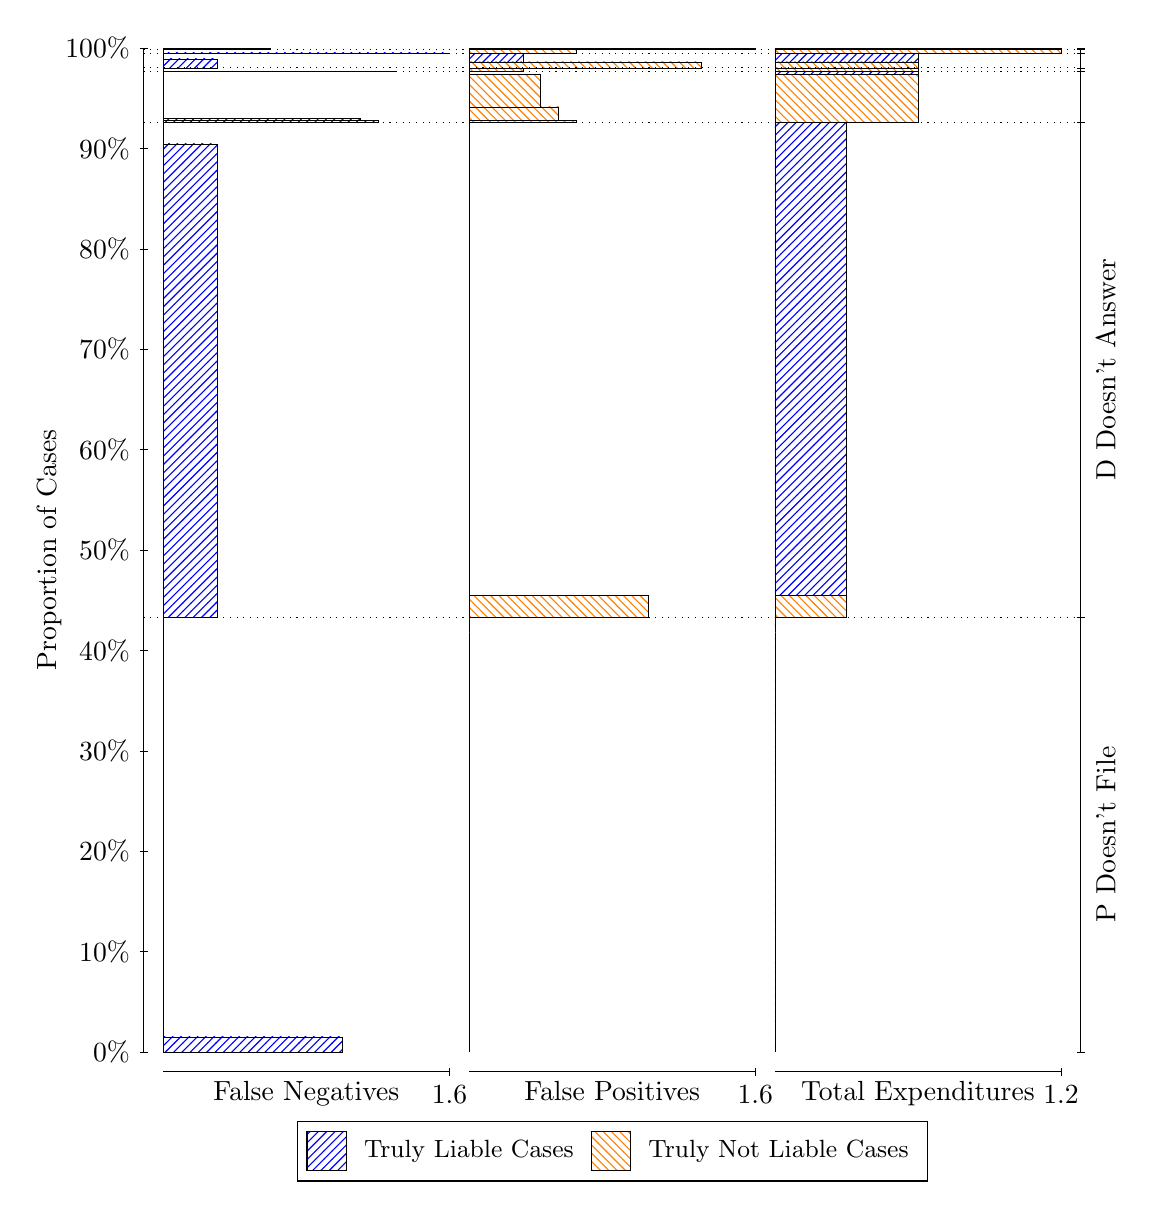
\begin{tikzpicture}
\draw[black, very thin] (1.5,1.75) -- (1.5,14.5);
\node[rotate=90, anchor=center] at (0.3, 8.125) {Proportion of Cases};
\draw[black, very thin] (1.45,1.75) -- (1.55,1.75);
\node[anchor=east] at (1.45, 1.75) {0\%};
\draw[black, very thin] (1.45,3.025) -- (1.55,3.025);
\node[anchor=east] at (1.45, 3.025) {10\%};
\draw[black, very thin] (1.45,4.3) -- (1.55,4.3);
\node[anchor=east] at (1.45, 4.3) {20\%};
\draw[black, very thin] (1.45,5.575) -- (1.55,5.575);
\node[anchor=east] at (1.45, 5.575) {30\%};
\draw[black, very thin] (1.45,6.85) -- (1.55,6.85);
\node[anchor=east] at (1.45, 6.85) {40\%};
\draw[black, very thin] (1.45,8.125) -- (1.55,8.125);
\node[anchor=east] at (1.45, 8.125) {50\%};
\draw[black, very thin] (1.45,9.4) -- (1.55,9.4);
\node[anchor=east] at (1.45, 9.4) {60\%};
\draw[black, very thin] (1.45,10.675) -- (1.55,10.675);
\node[anchor=east] at (1.45, 10.675) {70\%};
\draw[black, very thin] (1.45,11.95) -- (1.55,11.95);
\node[anchor=east] at (1.45, 11.95) {80\%};
\draw[black, very thin] (1.45,13.225) -- (1.55,13.225);
\node[anchor=east] at (1.45, 13.225) {90\%};
\draw[black, very thin] (1.45,14.5) -- (1.55,14.5);
\node[anchor=east] at (1.45, 14.5) {100\%};

\draw[black, very thin] (13.4,1.75) -- (13.4,14.5);
\draw[black, very thin] (13.35,1.75) -- (13.45,1.75);
\node[anchor=west] at (13.35, 1.75) {};
\draw[black, very thin] (13.35,7.2719) -- (13.45,7.2719);
\node[anchor=west] at (13.35, 7.2719) {};
\draw[black, very thin] (13.35,13.559) -- (13.45,13.559);
\node[anchor=west] at (13.35, 13.559) {};
\draw[black, very thin] (13.35,14.207) -- (13.45,14.207);
\node[anchor=west] at (13.35, 14.207) {};
\draw[black, very thin] (13.35,14.249) -- (13.45,14.249);
\node[anchor=west] at (13.35, 14.249) {};
\draw[black, very thin] (13.35,14.436) -- (13.45,14.436);
\node[anchor=west] at (13.35, 14.436) {};
\draw[black, very thin] (13.35,14.485) -- (13.45,14.485);
\node[anchor=west] at (13.35, 14.485) {};
\draw[black, very thin] (13.35,14.5) -- (13.45,14.5);
\node[anchor=west] at (13.35, 14.5) {};

\draw[black, very thin, pattern color=blue, pattern=north east lines] (1.75,1.75) rectangle (4.0208,1.9426);
\draw[black, very thin, pattern color=orange, pattern=north west lines] (1.75,1.9426) rectangle (1.75,7.2719);
\draw[black, very thin, pattern color=blue, pattern=north east lines] (1.75,7.2719) rectangle (2.4312,13.284);
\draw[black, very thin, pattern color=orange, pattern=north west lines] (1.75,13.284) rectangle (1.75,13.559);
\draw[black, very thin, pattern color=blue, pattern=north east lines] (1.75,13.559) rectangle (4.475,13.579);
\draw[black, very thin, pattern color=blue, pattern=north east lines] (1.75,13.579) rectangle (4.2479,13.602);
\draw[black, very thin, pattern color=blue, pattern=north east lines] (1.75,13.602) rectangle (4.0208,13.605);
\draw[black, very thin, pattern color=orange, pattern=north west lines] (1.75,13.605) rectangle (1.75,14.207);
\draw[black, very thin, pattern color=blue, pattern=north east lines] (1.75,14.207) rectangle (4.7021,14.208);
\draw[black, very thin, pattern color=orange, pattern=north west lines] (1.75,14.208) rectangle (1.75,14.249);
\draw[black, very thin, pattern color=blue, pattern=north east lines] (1.75,14.249) rectangle (2.4312,14.361);
\draw[black, very thin, pattern color=orange, pattern=north west lines] (1.75,14.361) rectangle (1.75,14.436);
\draw[black, very thin, pattern color=blue, pattern=north east lines] (1.75,14.436) rectangle (5.3833,14.439);
\draw[black, very thin, pattern color=orange, pattern=north west lines] (1.75,14.439) rectangle (1.75,14.485);
\draw[black, very thin, pattern color=blue, pattern=north east lines] (1.75,14.485) rectangle (3.1125,14.493);
\draw[black, very thin, pattern color=orange, pattern=north west lines] (1.75,14.493) rectangle (1.75,14.5);
\draw[black, very thin, pattern color=orange, pattern=north west lines] (5.6333,1.75) rectangle (5.6333,7.0793);
\draw[black, very thin, pattern color=blue, pattern=north east lines] (5.6333,7.0793) rectangle (5.6333,7.2719);
\draw[black, very thin, pattern color=orange, pattern=north west lines] (5.6333,7.2719) rectangle (7.9042,7.5469);
\draw[black, very thin, pattern color=blue, pattern=north east lines] (5.6333,7.5469) rectangle (5.6333,13.559);
\draw[black, very thin, pattern color=orange, pattern=north west lines] (5.6333,13.559) rectangle (6.9958,13.579);
\draw[black, very thin, pattern color=orange, pattern=north west lines] (5.6333,13.579) rectangle (6.7687,13.752);
\draw[black, very thin, pattern color=orange, pattern=north west lines] (5.6333,13.752) rectangle (6.5417,14.161);
\draw[black, very thin, pattern color=blue, pattern=north east lines] (5.6333,14.161) rectangle (5.6333,14.207);
\draw[black, very thin, pattern color=orange, pattern=north west lines] (5.6333,14.207) rectangle (6.3146,14.247);
\draw[black, very thin, pattern color=blue, pattern=north east lines] (5.6333,14.247) rectangle (5.6333,14.249);
\draw[black, very thin, pattern color=orange, pattern=north west lines] (5.6333,14.249) rectangle (8.5854,14.324);
\draw[black, very thin, pattern color=blue, pattern=north east lines] (5.6333,14.324) rectangle (6.3146,14.436);
\draw[black, very thin, pattern color=orange, pattern=north west lines] (5.6333,14.436) rectangle (6.9958,14.483);
\draw[black, very thin, pattern color=blue, pattern=north east lines] (5.6333,14.483) rectangle (5.6333,14.485);
\draw[black, very thin, pattern color=orange, pattern=north west lines] (5.6333,14.485) rectangle (9.2667,14.492);
\draw[black, very thin, pattern color=blue, pattern=north east lines] (5.6333,14.492) rectangle (6.9958,14.5);
\draw[black, very thin, pattern color=orange, pattern=north west lines] (9.5167,1.75) rectangle (9.5167,7.0793);
\draw[black, very thin, pattern color=blue, pattern=north east lines] (9.5167,7.0793) rectangle (9.5167,7.2719);
\draw[black, very thin, pattern color=orange, pattern=north west lines] (9.5167,7.2719) rectangle (10.425,7.5469);
\draw[black, very thin, pattern color=blue, pattern=north east lines] (9.5167,7.5469) rectangle (10.425,13.559);
\draw[black, very thin, pattern color=orange, pattern=north west lines] (9.5167,13.559) rectangle (11.333,14.161);
\draw[black, very thin, pattern color=blue, pattern=north east lines] (9.5167,14.161) rectangle (11.333,14.207);
\draw[black, very thin, pattern color=orange, pattern=north west lines] (9.5167,14.207) rectangle (11.333,14.247);
\draw[black, very thin, pattern color=blue, pattern=north east lines] (9.5167,14.247) rectangle (11.333,14.249);
\draw[black, very thin, pattern color=orange, pattern=north west lines] (9.5167,14.249) rectangle (11.333,14.324);
\draw[black, very thin, pattern color=blue, pattern=north east lines] (9.5167,14.324) rectangle (11.333,14.436);
\draw[black, very thin, pattern color=orange, pattern=north west lines] (9.5167,14.436) rectangle (13.15,14.483);
\draw[black, very thin, pattern color=blue, pattern=north east lines] (9.5167,14.483) rectangle (13.15,14.485);
\draw[black, very thin, pattern color=orange, pattern=north west lines] (9.5167,14.485) rectangle (13.15,14.492);
\draw[black, very thin, pattern color=blue, pattern=north east lines] (9.5167,14.492) rectangle (13.15,14.5);
\draw[black, dotted] (1.5,7.2719) -- (13.4,7.2719);
\draw[black, dotted] (1.5,13.559) -- (13.4,13.559);
\draw[black, dotted] (1.5,14.207) -- (13.4,14.207);
\draw[black, dotted] (1.5,14.249) -- (13.4,14.249);
\draw[black, dotted] (1.5,14.436) -- (13.4,14.436);
\draw[black, dotted] (1.5,14.485) -- (13.4,14.485);
\draw[black, very thin] (1.75,1.5) -- (5.3833,1.5);
\node[anchor=north] at (3.5667, 1.5) {False Negatives};
\draw[black, very thin] (5.3833,1.45) -- (5.3833,1.55);
\node[anchor=north] at (5.3833, 1.45) {1.6};

\draw[black, very thin] (5.6333,1.5) -- (9.2667,1.5);
\node[anchor=north] at (7.45, 1.5) {False Positives};
\draw[black, very thin] (9.2667,1.45) -- (9.2667,1.55);
\node[anchor=north] at (9.2667, 1.45) {1.6};

\draw[black, very thin] (9.5167,1.5) -- (13.15,1.5);
\node[anchor=north] at (11.333, 1.5) {Total Expenditures};
\draw[black, very thin] (13.15,1.45) -- (13.15,1.55);
\node[anchor=north] at (13.15, 1.45) {1.2};

\node[black, centered, rotate=90] at (13.72, 4.5109) {P Doesn't File};
\node[black, centered, rotate=90] at (13.72, 10.416) {D Doesn't Answer};






\draw (7.449999999999999,1.5) node[draw=none] (baseCoordinate) {};
\begin{scope}[align=center]
        \matrix[scale=0.5, draw=black, below=0.5cm of baseCoordinate, nodes={draw}, column sep=0.1cm]{
            \node[rectangle, draw, minimum width=0.5cm, minimum height=0.5cm, pattern=north east lines, pattern color=blue] {}; &
            \node[draw=none, font=\small] (B) {Truly Liable Cases}; &
            \node[rectangle, draw, minimum width=0.5cm, minimum height=0.5cm, pattern=north west lines, pattern color=orange] {}; &
            \node[draw=none, font=\small] (B) {Truly Not Liable Cases}; \\
            };
\end{scope}

\end{tikzpicture}
\end{document}